
As próximas seções discutem os modelos de dados NoSQL. Inicialmente é
feita a definição do termo NoSQL e, em seguida,
apresentamos diferentes formas de modelagem e armazenamento de bancos de
dados que guiam as atuais alternativas ao modelo relacional. Apesar de
discutirmos diferentes estratégias, o foco desse trabalho é comparar o
modelo relacional, amplamente usado pela indústria desde o início da
década de 90, com o modelo não relacional orientado a documentos. Por
essa razão, a Seção~\ref{sec:mongo} detalha o banco de dados orientado
a documentos MongoDB. 


\section{NoSQL}

O termo NoSql é a junção de duas palavras. \textit{No} e \textit{SQL}. Se traduzirmos de forma simplista, significa que é uma tecnologia/produto que trabalha de forma contrária à tecnologia dos banco relacionais (adeptos do SQL). O termo é usado com o sentido de Não Relacional. Atualmente o termo NoSql é traduzido para \textit{"Not only Sql"}, ou seja "Não só Sql".
Saindo da definição, NoSql é um termo genérico para uma classe definida de banco de dados não-relacionais que armazenam os dados  de forma diferente da conhecida modelagem relacional e que surgiram com o propósito de sanar algumas dificuldades encontradas com o modelo relacional. NoSql não é um produto, mas a uma classe de produtos e conceitos de armazenagem e manipulação de dados. 

O que diferencia os bancos de dados NoSql dos relacionais são os seus modelos de dados sem um \textit{schema} definido. Os bancos de dados NoSql podem ser classificados, segundo seu modelo de dados, em quatro grupos: chave-valor, orientados a documentos, orientados a colunas e baseados em grafos~\cite{nosqlxrelacional,nosqlevaluation}.

Bancos de dados que usam a modelagem não relacionais não são novidades. Conforme discutido no livro \emph{NoSql Professional}~\cite{nosqlprofessional} eles surgiram junto com as primeiras máquinas de computar. Bases não relacionais ficaram conhecidas e cresceram por causa do uso de \textit{mainframes} e em domínios específicos como o armazenamento de credenciais para autenticação. Esse NoSql que conhecemos hoje é uma nova visão, ou como diz Tiwari em \emph{NoSql Professional} ~\cite{nosqlprofessional}, uma reencarnação que nasceu no mundo de aplicações web que necessitam de recursos escaláveis para tratar de sua enorme massa de dados. Apesar de o paradigma NoSql já ter sido criado há algum tempo ele só tomou as proporções atuais depois que grandes empresas como Google, Amazon e Facebook começaram a usá-los em suas arquiteturas~\cite{nosqlevaluation}.

Ao utilizar SGBD's relacionais com grandes quantidades de dados surgem problemas como falta de eficiência no processamento, uma paralelização não efetiva, alto custo e escalabilidade limitada. Sendo um gigante da Internet, a Google,  se não for a empresa que manipula a maior quantidade de dados, é com certeza uma das maiores e ao se deparar com essa problemática  construiu a sua própria infraestrutura para que o seu mecanismo de busca e outras aplicações pudessem tratar a massa de dados de forma eficiente.

Com o lançamento de artigos pelo Google que explicavam em partes como o problema foi solucionado, desenvolvedores de \textit{software} livre criaram o primeiro motor de busca de código aberto que replicava algumas características da infraestrutura do Google, o Lucene. Logo depois, os principais desenvolvedores do Lucene se juntaram ao Yahoo e com a ajuda de diversos outros desenvolvedores criaram uma estrutura que imitava todas as peças da infraestrutura de computação distribuída do 
Google. Essa solução livre é o Hadoop. Nessa mesma época surgiu a ideia do NoSql. 

O sucesso do Google e o Hadoop ajudaram a impulsionar novos conceitos de computação distribuída, NoSql e o próprio projeto Hadoop. Um ano após o lançamento dos artigos do Google outra gigante da internet resolveu compartilhar o seu caso de sucesso. Em 2007 a Amazon mostrou ao mundo sua solução de base de dados distribuída, disponível e consistente que se chama Dynamo.

Após Google e Amazon mostrarem a aplicabilidade do NoSql, diversos
outros produtos surgiram nessa linha. O NoSql e os conceitos de manipulação de \textit{big data} ganharam espaço e foram surgindo diversos casos de uso de sucesso de grandes companhias como o Facebook, Netflix, Yahoo, EBay, Hulu, IBM e diversas outras.


\subsection{Modelos de Banco de Dados NoSql}


\subsubsection{Chave-Valor}

Bancos de dados NoSql que usam a modelagem Chave-Valor armazenam os dados indexados por um valor chave. A base é similar a um dicionário, onde os dados são endereçados por uma única chave. Uma vez que os dados são armazenados, é através das suas chaves a única forma de recuperá-los. Os valores são isolados e independentes um dos outros, sendo necessário tratar isso na aplicação. Por isso os bancos chave-valor são livres de \textit{schema}. Isso permite que novos tipos de dados sejam inseridos em tempo de execução sem que o banco entre em conflito e sem influenciar na disponibilidade do sistema~\cite{nosqlevaluation,nosqlliveup}.

Alguns exemplos de banco de dados que usam esse tipo de modelagem são: RIAK, LevelDB, Voldemort, redis~\cite{nosqldatabaseorg}.

\subsubsection{Orientados a Documentos}

A modelagem orientada a documentos armazena os dados encapsulados em pares de chave-valor em JSON ou em outro padrão semelhante. Dentro dos documentos as chaves devem ser únicas. Cada documento recebe um identificador que também é único dentro de uma coleção de documentos. Os documentos são as unidades básicas e não têm uma estrutura definida como nas tabelas do modelo relacional, ou seja, não tem um \textit{schema} de dados definido. Ao armazenar os dados em JSON há uma vantagem adicional que é o suporte a tipos de dados, o que torna a forma de armazenamento mais amigável para os desenvolvedores~\cite{nosqlevaluation,nosqlxrelacional}. O exemplo de codificação \ref{listing:excouchdb} nos mostra como é a estrutura desse tipo de banco de dados.

Os exemplos mais significativos são: CouchDB, MongoDB e Riak~\cite{nosqlevaluation}.

	\begin{lstlisting}[caption=Exemplo de arquivo do CouchDB, frame=trBL,breaklines=true,label=listing:excouchdb]

{
    "Subject": "I like Plankton",
    "Author": "Rusty",
    "PostedDate": "5/23/2006",
    "Tags": ["plankton", "baseball", "decisions"],
    "Body": "I decided today that I don't like baseball. I like plankton."
}
	\end{lstlisting}

\subsubsection{Orientados a Colunas}

Nesse tipo de modelagem o paradigma passa a ser de orientação a atributos(colunas). Ao contrário da modelagem chave-valor, agora os dados são armazenados usando tabelas sem um \textit{schema} definido, mas sem suporte a associação entre elas . Figura ~\ref{fig:mdcolumns} Segundo Jing Han et all, um banco orientado a colunas tem as seguintes características ~\cite{surveynosql}:


\begin{enumerate}
\item{Os dados são armazenados em colunas}
\item{Cada coluna de dado é um índice do banco}
\item{Acessar somente colunas faz com que haja redução de I/O nos resultados das consultas}
\item{Consultas simultâneas, isto é, cada coluna é tratada por um processo}
\item{Possuem o mesmo tipo de dados, características semelhantes e boa taxa de compressão}
\end{enumerate}

Em geral esse tipo de banco é mais vantajoso para aplicações de agregação e data warehouses. Alguns exemplos são: Cassandra e  Hypertable ~\cite{nosqldatabaseorg}.



	\begin{figure}[!htbp]
		\begin{center}
			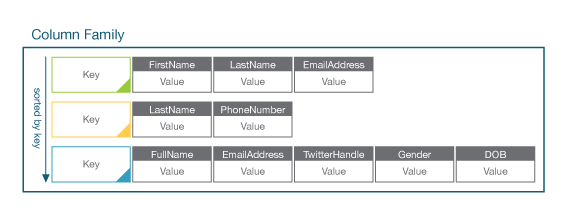
\includegraphics[width=0.8\textwidth]{columns}
		\end{center}
		\caption{Modelagem orientada a colunas}
		\label{fig:mdcolumns}
	\end{figure}


\subsubsection{Baseados em Grafos}

Nessa categoria os dados são armazenados em nós de um grafo cujas arestas representam o tipo de associação entre esses nós. Esse tipo de banco é especializado em manter dados fortemente ligados. O twitter armazena as relações entre os seus usuários no seu próprio banco de dados baseados em grafos, o FlockDB, que é otimizado para listas de relações muito grandes, leituras e escritas~\cite{nosqlevaluation}.  Alguns exemplos são: Neo4J, infoGrid e FlockDB~\cite{nosqldatabaseorg}.

\subsection{MongoDB}\label{sec:mongo}

Essa seção foi baseada no site oficial do MongoDB~\cite{sitemongodb} exceto quando explicitamente citado.
MongoDB é um banco de dados NoSQL,  de código aberto,  orientado a documentos, \textit{schema-free} e escrito em C++.  Os dados são persistidos em coleções de dados que são representados usando o BSON, um formato binário similar ao JSON (Figura \ref{fig:exbson}). O MongoDB tem suporte a todos os tipos de dados  JSON  como string, inteiro, boleano, double, array e objeto. Por usar codificação BSON o MongoDB suporta alguns tipo de dados adicionais como data, binary data, regular expression e code ~\cite{nosqlprofessional}. Na Figura \ref{tab:bytes} podemos ver os tipos suportados pelo BSON.

\begin{table}
	\caption{BSON - Tipos Suportados}
	\begin{center}
	\begin{tabular}{ccc}
		\hline
			\textbf{Tipo} & \textbf{Número} \\
		\hline
			Double & 1 \\
			String & 2 \\
			Object & 3 \\
			Array & 4 \\
			Binary Data & 5 \\
			Object id & 7 \\
			Boolean & 8 \\
			Date & 9 \\
			Null & 10 \\
			Regular Expression & 11 \\
			JavaScript & 13 \\
			Symbol & 14 \\
			JavaScript (with scope) & 15 \\
			32-bit integer & 16 \\
			Timestamp& 17 \\
			64-bit integer & 18 \\
			Min key & 255 \\
			Max key & 127 \\
		\hline
	\end {tabular}
	\end{center}
	%\caption{Fonte: http://docs.mongodb.org}
	\label{tab:bsontypes}
\end{table}

Como não usa o mesmo formato de armazenamento dos SGBDs relacionais, o MongoDB armazena os seus dados em coleções, que são equivalentes às tabelas.  Uma Coleção pode ter um ou mais documentos; são equivalentes as linhas em uma tabela de um banco de dados relacional. Cada documento tem um ou mais campos, o que corresponde a uma coluna.

Diferente do que a maioria das pessoas estão acostumadas, o MongoDB não trabalha com uma estrutura de dados bem definida (\textit{schema}), ou melhor dizendo, ele usa \textit{schemas} dinâmicos. Com ele é possível criar coleções sem que a estrutura, campos ou tipos de valores dos documentos estejam definidos. Essa forma flexível de armazenar os dados nos permite trabalhar com estruturas e dados bastante heterogêneos.

	\begin{figure}[!htbp]
		\begin{center}
			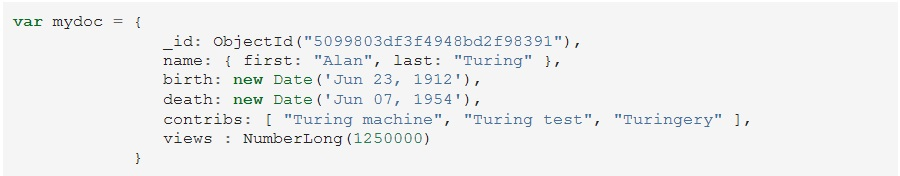
\includegraphics[width=1.2\textwidth]{exbson}
		\end{center}
		\caption{Documento BSON usado no MongoDB ~\cite{sitemongodb}}
		\label{fig:exbson}
	\end{figure}

Quanto mais controle, mais custosa é uma operação para o sistema gerenciador de banco de dados.  Os bancos de dados NoSQL, como dito anteriormente, foram criados para suprir algumas características que os bancos de dados relacionais não atendiam. Uma dessas características é a velocidade com que operações de consulta, escrita, atualização e exclusão são executadas.  Para que a velocidade dessas transações fosse aumentada foi preciso retirar alguns controles e, com isso, os bancos de dados NoSQL não se comprometem com todas as características ACID.

O MongoDB não provê transações ACID, mas possui alguns recursos transacionais básicos. Operações atômicas são possíveis no escopo de um único documento. Na tabela abaixo temos alguns exemplos de operações em SQL e suas correspondentes no MongoDB.

\subsubsection{Modelagem dos Dados}

Cada documento tem um campo chamado ID que é utilizado como chave primária. Para aumentar a velocidade das \textit{queries} é possível habilitar índices para os campos que são utilizados nas consultas. O MongoDB também suporta índices em sub-documentos e em arrays.

Ao contrário dos bancos de dados convencionais o MongoDB possui um \textit{schema} flexível e não nos força a determinar uma estrutura antes de inserir os dados. As coleções no MongoDB não nos impedem de evoluir a estrutura dos documentos ~\cite{Orendanalysisand}.

Para representar as relações entre os objetos temos duas estratégias: referências e sub-documentos ~\cite{Orendanalysisand}. O modelo implementado no protótipo utilizado para a realização dos testes pode ser visto na Figura \ref{fig:modeloorientadodocumentos} e utiliza as duas estratégias de modelagem.

	\begin{figure}[!htbp]
		\begin{center}
			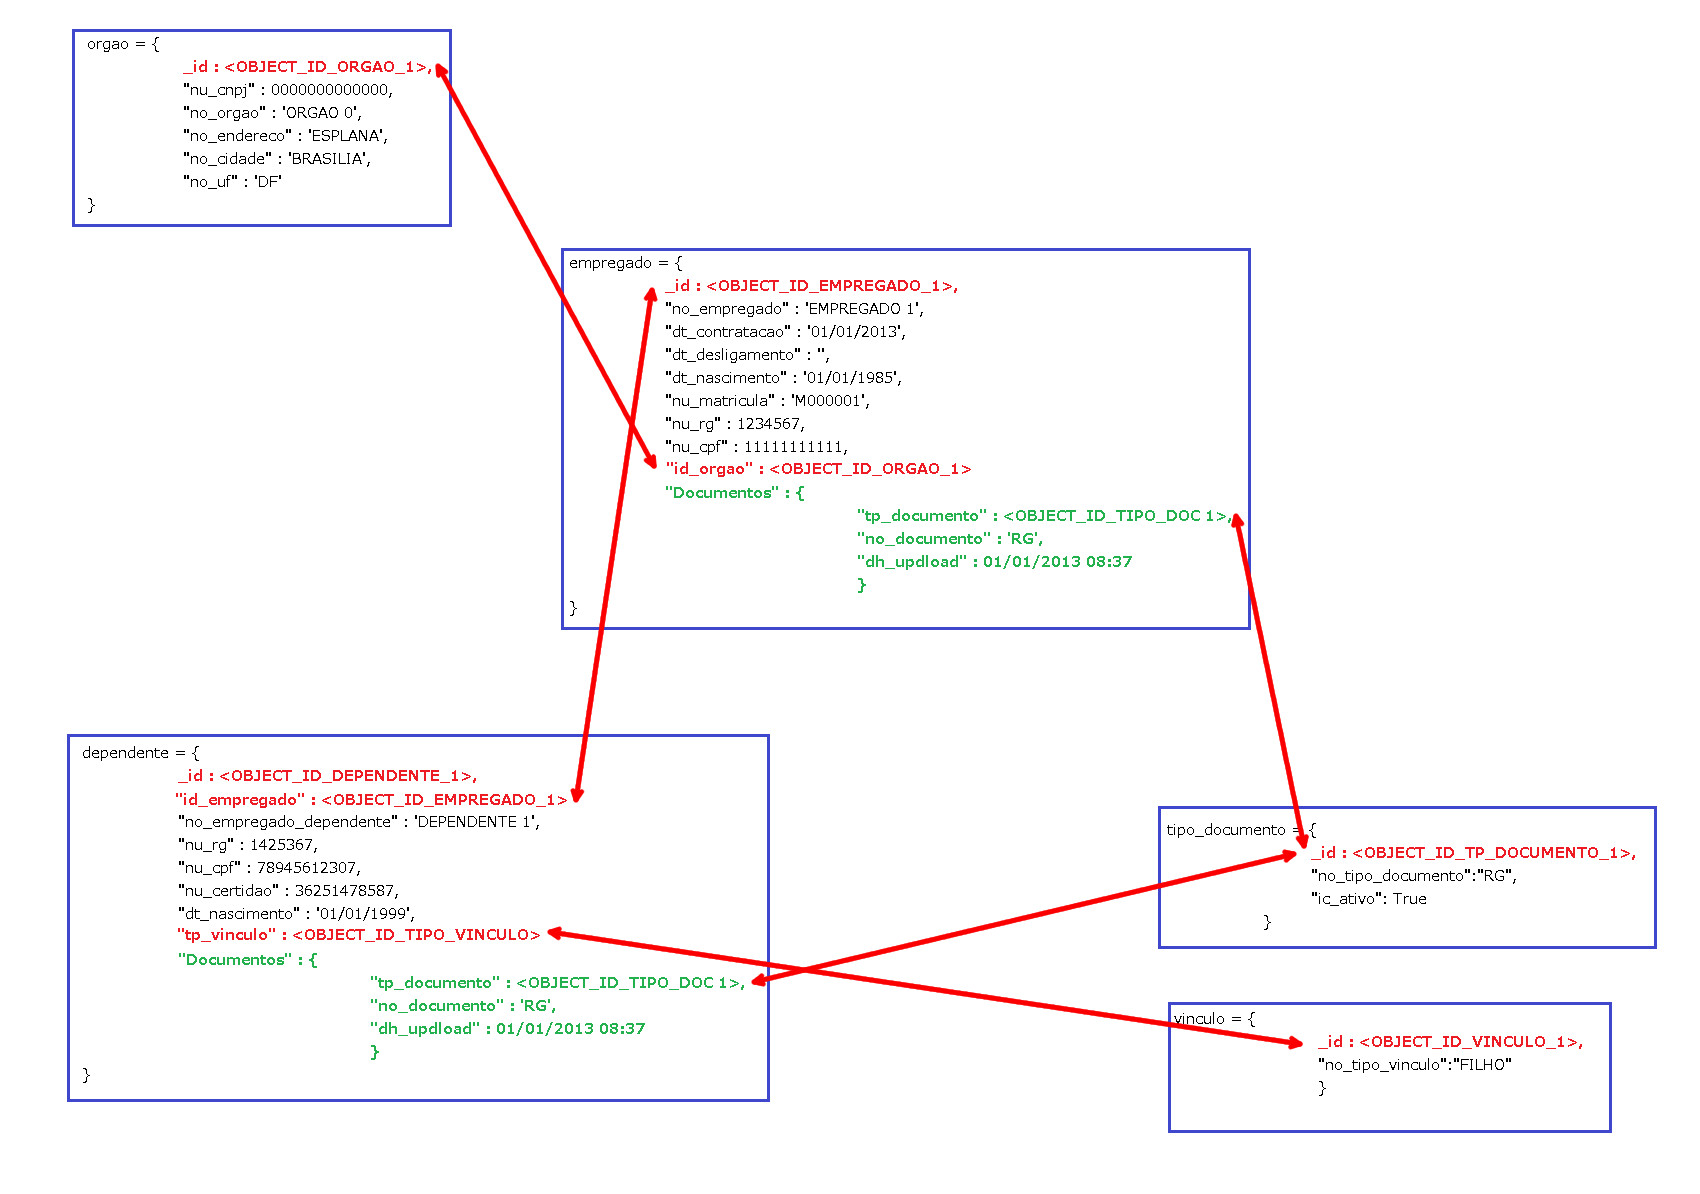
\includegraphics[width=1.4\textwidth, angle=-90]{modelo_orientado_documentos}
		\end{center}
		\caption{ Modelagem orientada a documentos implementada no protótipo.}
		\label{fig:modeloorientadodocumentos}
	\end{figure}

%\subsubsection{Referências}

O referenciamento representa as relações entre os dados incluindo \textit{links} ou referências de um documento para outro. Para acessar os dados referenciados a aplicação deve resolver a referência. Na Figura \ref{fig:referencia}, temos um exemplo de modelagem utilizando referência.

	\begin{figure}[!htbp]
		\begin{center}
			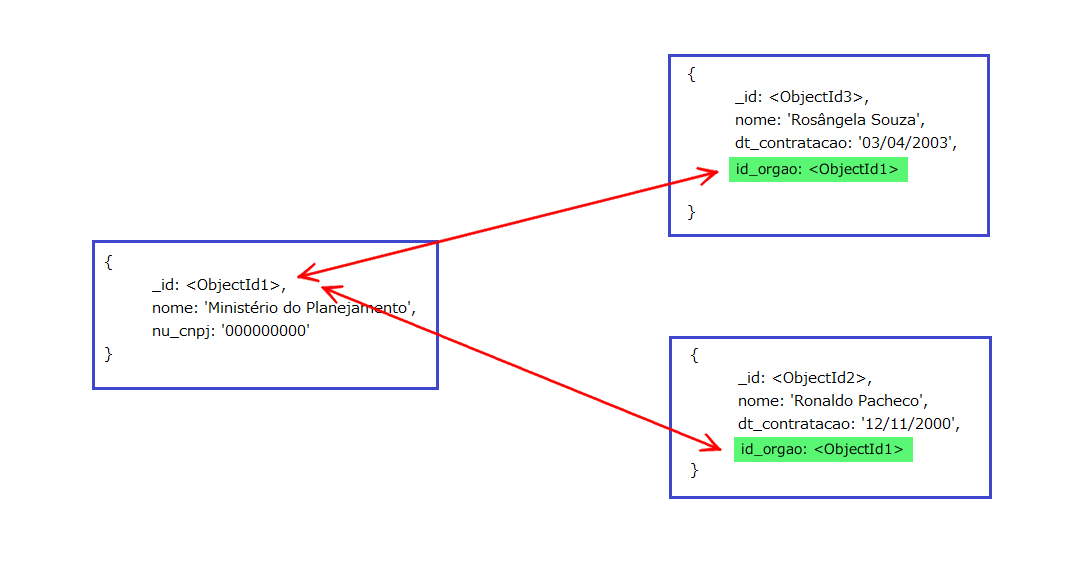
\includegraphics[width=0.8\textwidth]{referencia}
		\end{center}
		\caption{ Modelagem utilizando referência. Adaptado de ~\cite{sitemongodb}}
		\label{fig:referencia}
	\end{figure}

Seguem algumas ocasiões em que podemos utilizar referências como estratégia de modelagem:

\begin{itemize}
	\item Quando, ao criar sub-documentos, criamos duplicação de dados e essa duplicação não nos dá um ganho de performance vantajoso.
	\item Quando desejamos representar complexas relações de n para n.
	\item Para representar um grande volume de dados de forma hierárquica.
\end{itemize}

Ao implementar as referências temos mais flexibilidade se compararmos com os sub-documentos. Em contrapartida, ao realizarmos consultas, essas referências deverão ser traduzidas, o que gera mais consultas ao servidor ~\cite{Orendanalysisand}.

%\subsubsection{Sub-Documentos}

A outra estratégia possível é o uso de sub-documentos. Ao utilizar essa forma de armazenamento os dados relacionados são armazenados em um único documento. O MongoDB permite armazenar essas relações em sub-documentos ou arrays de documentos. Veja um exemplo desse tipo de modelagem na Figura \ref{fig:subdocumento}.

	\begin{figure}[!htbp]
		\begin{center}
			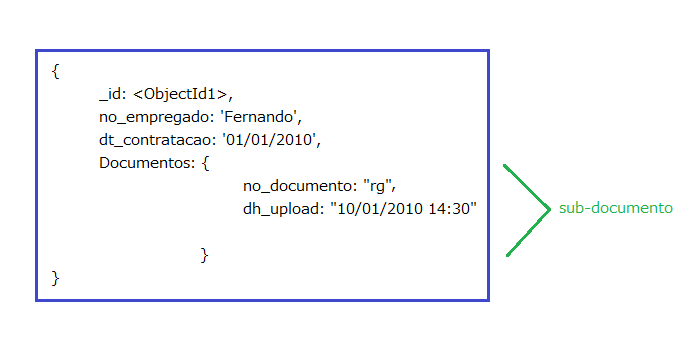
\includegraphics[width=0.8\textwidth]{subdocumento}
		\end{center}
		\caption{ Modelagem utilizando sub-documento. Adaptado de ~\cite{sitemongodb}}
		\label{fig:subdocumento}
	\end{figure}

Seguem algumas ocasiões em que podemos utilizar os sub-documentos:

\begin{itemize}
	\item Em relações um para um;
	\item Em relações um para muitos. Nesses relacionamentos o objeto que se repete deve estar contido no outro objeto;
\end{itemize}

Os sub-documentos aumentam a performance de operações de leitura e nos dá a vantagem de obter os dados necessários em uma simples consulta ao banco. Com os sub-documentos também é possível realizar atualizações de forma atômica ~\cite{Orendanalysisand}.

\subsubsection{Linguagem de Consulta}

A sintaxe da linguagem de consulta do MongoDB é similar ao JSON. A linguagem de consulta permite consultar todos os documentos em uma coleção, inclusive os sub-documentos e os arrays ~\cite{Orendanalysisand}.

A linguagem de consulta suporta ~\cite{Orendanalysisand}]:
\begin{itemize}
	\item Consultas em documentos e sub-documentos
	\item Comparações
	\item Operações lógicas
	\item Ordenação por múltiplos campos
	\item \textit{Group by}
	\item Uma agregação por consulta
\end{itemize}

Adicionalmente o MongoDB permite realizar consultas com agregações mais complexas utilizando uma variação do MapReduce ~\cite{Orendanalysisand}.

Nas tabelas \ref{tab:sqlvsmongo} e  \ref{tab:sqlvsmongoselect} temos algumas comparações entre a linguagem utilizada pelo MongoDB e o SQL.

\begin{table}[h]
	\caption{Declarações SQL vs Declarações MongoDB. Adaptado de ~\cite{sitemongodb}}
	\begin{center}
	\begin{tabular}{  l   p{8cm} }
		\hline
			\textbf{SQL} & \textbf{MongoDB} \\
		\hline
\lstset{language=SQL}
\begin{lstlisting}
CREATE TABLE users (
	id MEDIUMINT NOT NULL
		AUTO_INCREMENT,
	user_id Varchar(30),
	age Number,
	status char(1),
	PRIMARY KEY (id)
)
\end{lstlisting}
 & O documento é criado na primeira operação de inserção. Se o campo id não for especificado ele é automaticamente gerado.
\lstset{language=Java}
\begin{lstlisting}
db.users.insert( {
    user_id: "abc123",
    age: 55,
    status: "A"
 } )
\end{lstlisting}
\\ \hline
\lstset{language=SQL}
\begin{lstlisting}
ALTER TABLE users
ADD join_date DATETIME
\end{lstlisting}
 & O MongoDB não fixa a estrutura das coleções. Não existe alteração estrutural no nivel das coleções. As alterações ocorrem no nível dos documentos.
\lstset{language=Java}
\begin{lstlisting}
db.users.update(
    { },
    { $set: { join_date: new Date() } },
    { multi: true }
)
\end{lstlisting}
\\ \hline
\lstset{language=SQL}
\begin{lstlisting}
ALTER TABLE users
DROP COLUMN join_date
\end{lstlisting}
&
\lstset{language=Java}
\begin{lstlisting}
db.users.update(
    { },
    { $unset: { join_date: "" } },
    { multi: true }
)
\end{lstlisting}
\\ \hline
\lstset{language=SQL}
\begin{lstlisting}
DROP TABLE users
\end{lstlisting}
&
\lstset{language=Java}
\begin{lstlisting}
db.users.drop()
\end{lstlisting}
\\ \hline
	\end {tabular}
	\end{center}
	\label{tab:sqlvsmongo}
\end{table}

\begin{table}[h]
	\caption{SQL Select vs MongoDB Select. Adaptado de ~\cite{sitemongodb}}
	\begin{center}
	\begin{tabular}{  l   p{8cm} }
		\hline
			\textbf{SQL} & \textbf{MongoDB} \\
		\hline
\lstset{language=SQL}
\begin{lstlisting}
SELECT *
FROM users
\end{lstlisting}
 &
\lstset{language=Java}
\begin{lstlisting}
db.users.find()
\end{lstlisting}
\\ \hline
\lstset{language=SQL}
\begin{lstlisting}
SELECT id, user_id, status
FROM users
\end{lstlisting}
 &
\lstset{language=Java}
\begin{lstlisting}
db.users.find(
    { },
    { user_id: 1, status: 1 }
)
\end{lstlisting}
\\ \hline
\lstset{language=SQL}
\begin{lstlisting}
SELECT *
FROM users
WHERE status = "A"
\end{lstlisting}
&
\lstset{language=Java}
\begin{lstlisting}
db.users.find(
    { status: "A" }
)
\end{lstlisting}
\\ \hline
\lstset{language=SQL}
\begin{lstlisting}
SELECT *
FROM users
WHERE status = "A"
AND age = 50
\end{lstlisting}
&
\lstset{language=Java}
\begin{lstlisting}
db.users.find(
    { status: "A",
      age: 50 }
)
\end{lstlisting}
\\ \hline
\lstset{language=SQL}
\begin{lstlisting}
SELECT COUNT(*)
FROM users
\end{lstlisting}
&
\lstset{language=Java}
\begin{lstlisting}
db.users.count()
\end{lstlisting}

ou

\begin{lstlisting}
db.users.find().count()
\end{lstlisting}
\\ \hline
\lstset{language=SQL}
\begin{lstlisting}
EXPLAIN SELECT *
FROM users
WHERE status = "A"
\end{lstlisting}
&
\lstset{language=Java}
\begin{lstlisting}
db.users.find( { status: "A" } ).explain()
\end{lstlisting}
\\ \hline
	\end {tabular}
	\end{center}
	\label{tab:sqlvsmongoselect}
\end{table}



\subsubsection{Replicação}

Replicação é o processo de sincronizar dados através de diferentes servidores. Com a replicação é possível prover redundância e aumentar a disponibilidade dos dados, além de proteger os dados de uma possível falha de \textit{hardware} ou catástrofes.

Um conjunto de réplicas é um grupo de instâncias do MongoDB com os mesmos dados. Na arquitetura de um conjunto de replicação somente um servidor, o primário, recebe todas as requisições de escrita. Os outros servidores somente replicam as operações em suas instâncias. A Figura \ref{fig:replication} representa a arquitetura para replicação.

Como somente um nó recebe todas as operações de escrita, para suportar a replicação, o nó primário armazena em \textit{log} todas as operações. Os nós secundários replicam os \textit{logs} do nó primário e, em seguida, realizam as operações em suas instâncias. Caso o nó primário fique indisponível, o conjunto de replicação eleje um novo nó para ser o primário. Por padrão, as requisições de leitura são feitas ao nó primário, porém isso pode ser alterado. Como a replicação é assíncrona, se as preferências de leitura forem alteradas os dados retornados podem não ser os mais atuais.

	\begin{figure}[!htbp]
		\begin{center}
			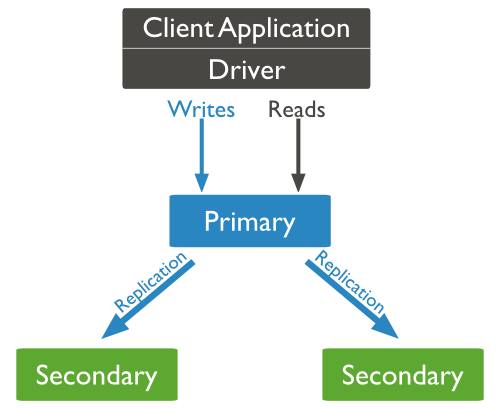
\includegraphics[width=0.5\textwidth]{replication}
		\end{center}
		\caption{Arquitetura de Replicação ~\cite{sitemongodb}}
		\label{fig:replication}
	\end{figure}


\subsubsection{Decomposição (Sharding)}

\textit{Sharding}, ou decomposição, é quando separamos a localização física dos dados, despedaçando cada informação e colocando-as em nós diferentes. Essa técnica é utilizada para trabalhar com dados de grande volume e com alta vazão de operações. A decomposição é a alternativa à escalabilidade vertical. No MongoDB a decomposição é implementada com o uso de um \textit{cluster} de decomposição. Os componentes desse \textit{cluster} são: \textit{Shards}, roteadores de consulta e servidores de configuração (Figura \ref{fig:sharding}).

Os \textit{shards} armazenam os dados.

Os roteadores de consulta, ou mongos, se comunicam com os clientes e direcionam as operações ao \textit{shard} ou \textit{shards} apropriados.

Os servidores de configuração armazenam os metadados do \textit{cluster}. Ele contém o mapa do \textit{cluster}. O roteador de consulta utiliza esse componente para encontrar os \textit{shards} que serão utilizados.

	\begin{figure}[!htbp]
		\begin{center}
			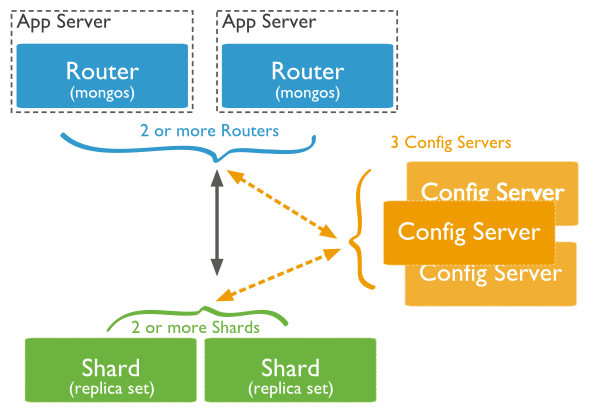
\includegraphics[width=0.5\textwidth]{sharding}
		\end{center}
		\caption{Cluster de Sharding ~\cite{sitemongodb}}
		\label{fig:sharding}
	\end{figure}

\subsubsection{Tratamento de Falhas}

O MongoDB não utiliza \textit{log}  de transações para garantir a durabilidade dos dados. E por utilizar arquivos mapeados em memória, implementa escrita preguiçosa (\textit{lazy write}). Sendo asssim, se um nó MongoDB falhar, provavelmente algum dado será perdido ~\cite{Orendanalysisand}.